% (a) one generated example in both renderings, (b) the headline accuracy curve.
\definecolor{formalcol}{RGB}{40,104,178}
\definecolor{natcol}{RGB}{34,139,94}

\begin{figure}[t]
\centering
\begin{subfigure}[t]{0.63\linewidth}
\centering
\begin{tikzpicture}[
  font=\tiny,
  box/.style={rounded corners=2pt, draw=gray!55, line width=0.5pt, inner sep=2.5pt, align=left},
  shared/.style={box, fill=gray!7},
  fbox/.style={box, draw=formalcol!65, fill=formalcol!5},
  nbox/.style={box, draw=natcol!65, fill=natcol!5},
  ar/.style={-{Latex[length=4pt,width=3.5pt]}, draw=gray!60, line width=0.5pt},
]
\node[shared, text width=0.93\linewidth] (prompt)
  {\textbf{Prompt}\quad \texttt{c3 is ruby. c3 is north. c7 is olive.}\\
   \texttt{If c3 is north and c3 is ruby, then c9 is teal.}\\
   \texttt{If c9 is teal, then c9 is west.}\\
   \texttt{If c9 is west and c7 is olive, then c4 is amber.}\\
   \texttt{What is c4?}};

\node[shared, below=2mm of prompt, text width=0.93\linewidth] (proof)
  {\textbf{Latent proof}\quad
   \texttt{Rc3}, \texttt{Nc3} $\Rightarrow$ \texttt{Tc9} $\Rightarrow$ \texttt{Wc9},
   with \texttt{Oc7} $\Rightarrow$ \texttt{Ac4}};

\node[fbox, below=4mm of proof.south west, anchor=north west, text width=0.44\linewidth] (formal)
  {\textcolor{formalcol}{\textbf{\textsc{Formal} target}}\\[1pt]
   \texttt{<premises>}\\
   \texttt{\ R c3 ; N c3 ; O c7}\\
   \texttt{\ N c3 \& R c3 -> T c9}\\
   \texttt{\ T c9 -> W c9}\\
   \texttt{\ W c9 \& O c7 -> A c4}\\
   \texttt{</premises>}\\
   \texttt{<proof> R c3 ; premise}\\
   \texttt{\ N c3 ; premise}\\
   \texttt{\ N c3 \& R c3 ; \&I,2,1}\\
   \texttt{\ T c9 ; ->E,3}\\
   \texttt{\ W c9 ; ->E,4}\\
   \texttt{\ O c7 ; premise}\\
   \texttt{\ W c9 \& O c7 ; \&I,5,6}\\
   \texttt{\ A c4 ; ->E,7 </proof>}\\
   \texttt{<answer> amber </answer>}};

\node[nbox, below=4mm of proof.south east, anchor=north east, text width=0.44\linewidth] (nat)
  {\textcolor{natcol}{\textbf{\textsc{English} target}}\\[1pt]
   \texttt{<think>}\\
   \texttt{\ c3 is ruby and c3 is north.}\\
   \texttt{\ Since c3 is north and c3 is}\\
   \texttt{\ ruby, c9 is teal.}\\
   \texttt{\ Since c9 is teal, c9 is west.}\\
   \texttt{\ c7 is olive.}\\
   \texttt{\ Since c9 is west and c7 is}\\
   \texttt{\ olive, c4 is amber.}\\
   \texttt{\ Therefore, c4 is amber.}\\
   \texttt{</think>}\\
   \texttt{<answer> amber </answer>}};

\draw[ar] (prompt) -- (proof);
\draw[ar] (proof.south) -- ++(0,-2mm) -| (formal.north);
\draw[ar] (proof.south) -- ++(0,-2mm) -| (nat.north);
\end{tikzpicture}
\caption{One generated example. The program samples a latent proof and writes
it out in either notation, so the prompt, the answer and the proof graph are
common to the two renderings.}
\label{fig:overview-a}
\end{subfigure}
\hfill
\begin{subfigure}[t]{0.34\linewidth}
\centering
\vspace{0pt}
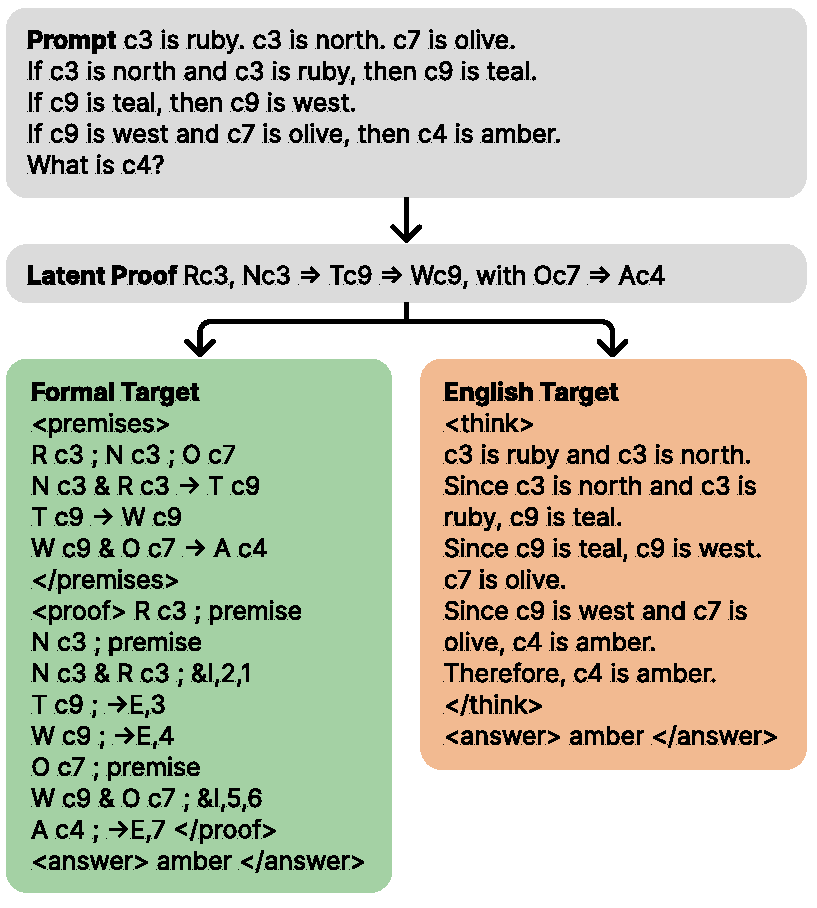
\includegraphics{figures/example.pdf}
\caption{Main results on Qwen2.5-7B. ProofWriter at
inference depth 3, FOLIO, the eight chain subtasks of BIG-Bench Hard, the 73
GPQA-Diamond items that ask for a computed value, and the share of generated
problems at chain length 25 on which the checker accepts the derivation.}
\label{fig:overview-b}
\end{subfigure}
\caption{The data added to the instruction mixture and what it buys. A
program writes the example on the left, which carries no world knowledge, and
replacing ten percent of the instruction mixture with such examples produces
the gains on the right. Table~\ref{tab:main} gives the full share sweep.}
\label{fig:overview}
\end{figure}
